\section{Extra Figures}\label{appendix 2}
\begin{figure}[h]
 \centering
 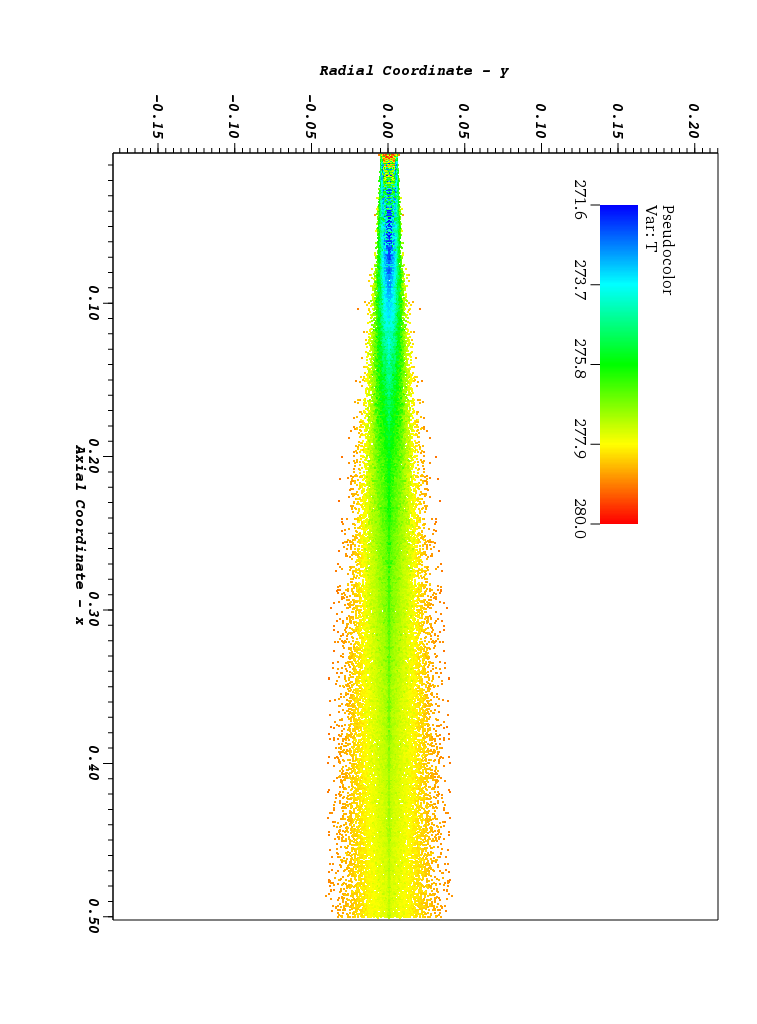
\includegraphics[height=0.7\textheight]{./figuras/appA2/visit_Td.png}
 % k_bc.png: 800x493 pixel, 100dpi, 20.32x12.52 cm, bb=
 \caption{Temperature of droplets. The computational domain is only half of the shown above, it is here mirrored for visualization purpose.}
 \label{fig: dropT}
\end{figure}

\clearpage
\begin{figure}
 \centering
 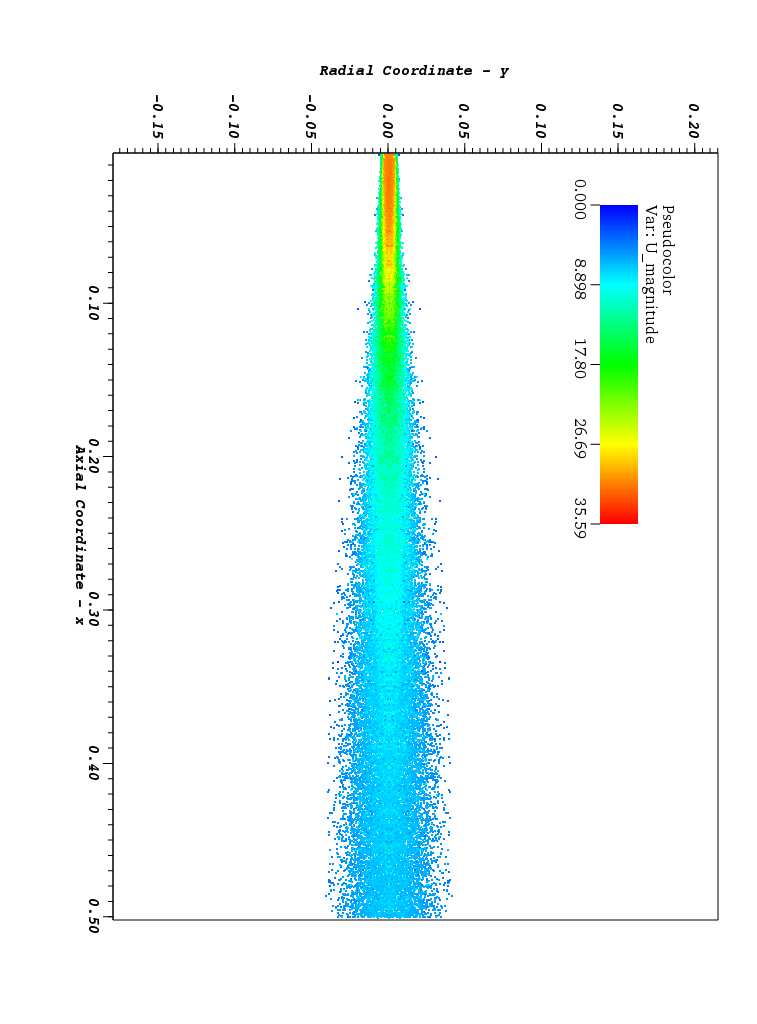
\includegraphics[height=0.9\textheight]{./figuras/appA2/visit_U.png}
 \caption{Magnitude of droplet velocities. The computational domain is only half of the shown above, it is here mirrored for visualization purpose.}
 \label{fig: dropU}
\end{figure}

\clearpage
\begin{figure}
\begin{center}
  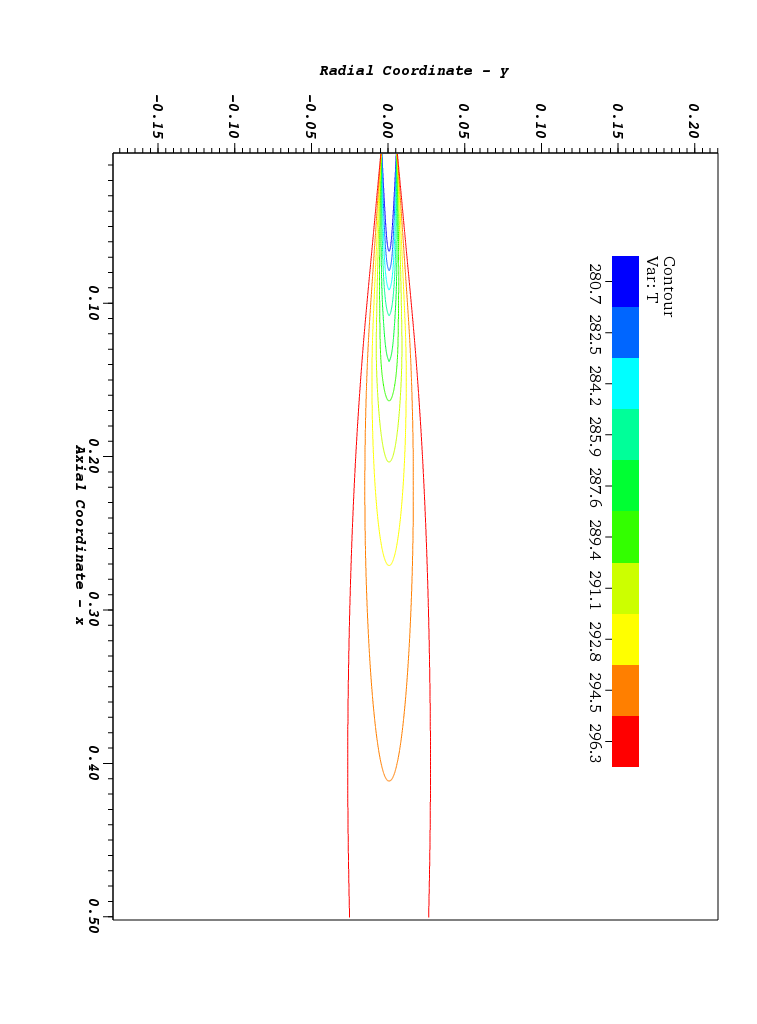
\includegraphics[height=0.9\textheight]{./figuras/appA2/visit_T.png}
 \end{center}
 \caption{Gas mean temperature field $\tilde{T}$. The computational domain is only half of the shown above, it is here mirrored for visualization purpose.}
 \label{fig: field_T}
\end{figure}

\clearpage
\begin{figure}
\begin{center}
  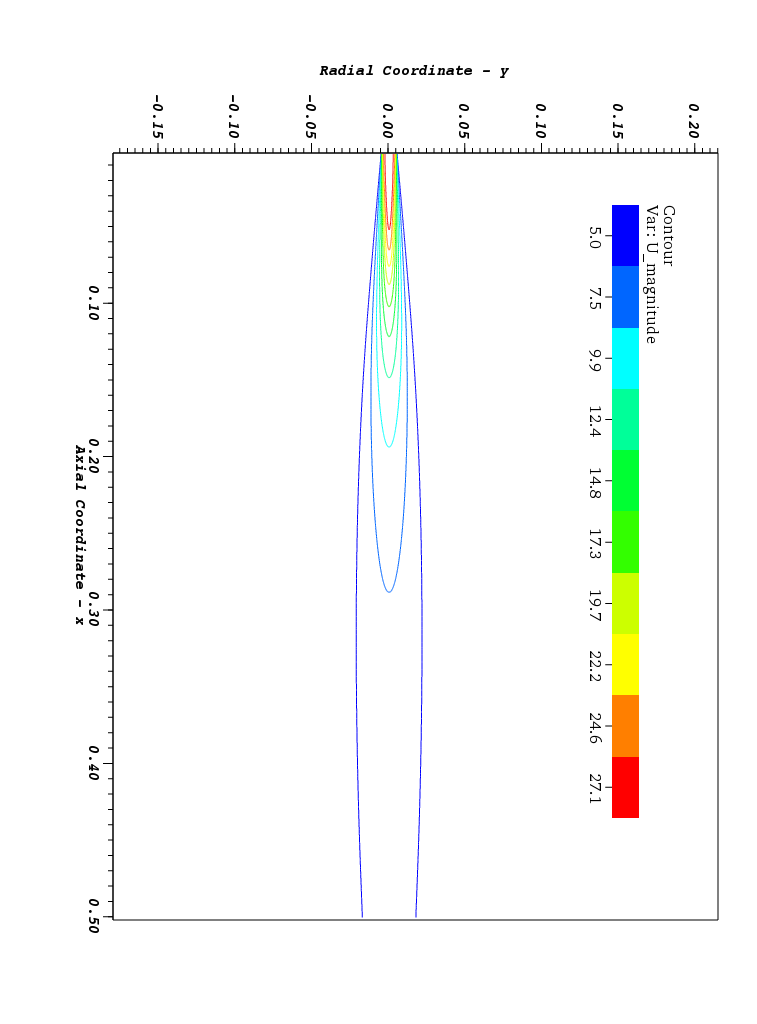
\includegraphics[height=0.9\textheight]{./figuras/appA2/visit_Ux.png}
 \end{center}
\caption{Gas mean velocity magnitude $|\tilde{\bv{U}}|$. The computational domain is only half of the shown above, it is here mirrored for visualization purpose.}
 \label{fig: field_U}
\end{figure}

\clearpage
\begin{figure}
\begin{center}
  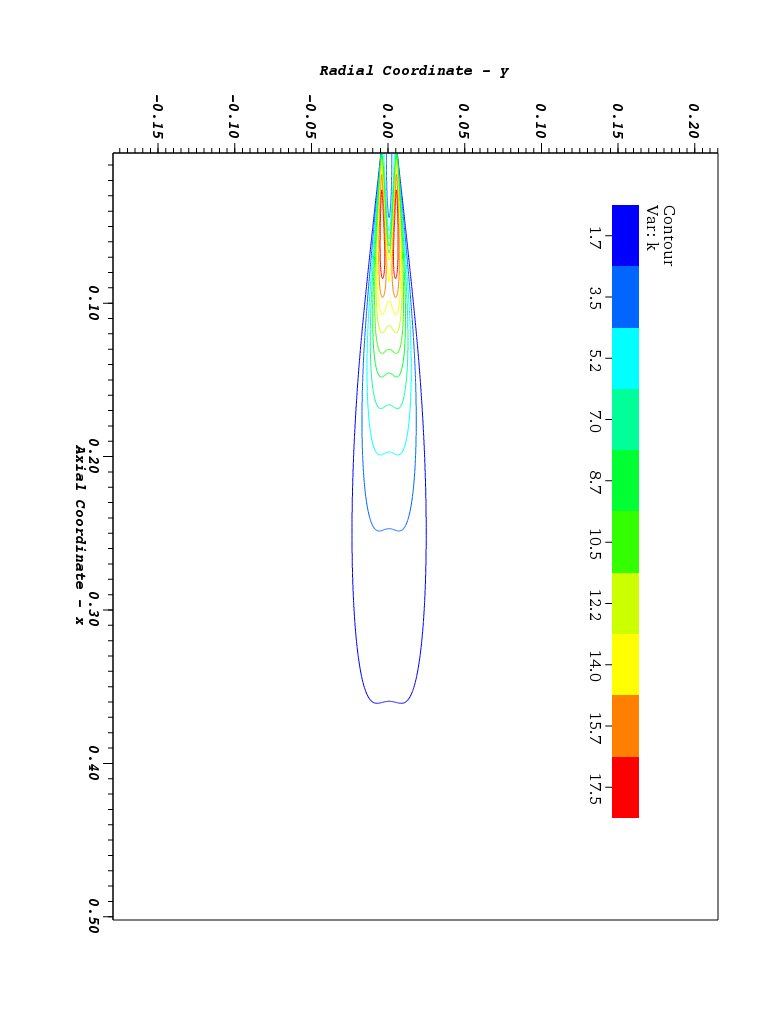
\includegraphics[height=0.9\textheight]{./figuras/appA2/visit_k.png}
 \end{center}
 \caption{Gas mean turbulent kinetic energy. The computational domain is only half of the shown above, it is here mirrored for visualization purpose.}
 \label{fig: field_k}
\end{figure}

\clearpage
\begin{figure}
\begin{center}
  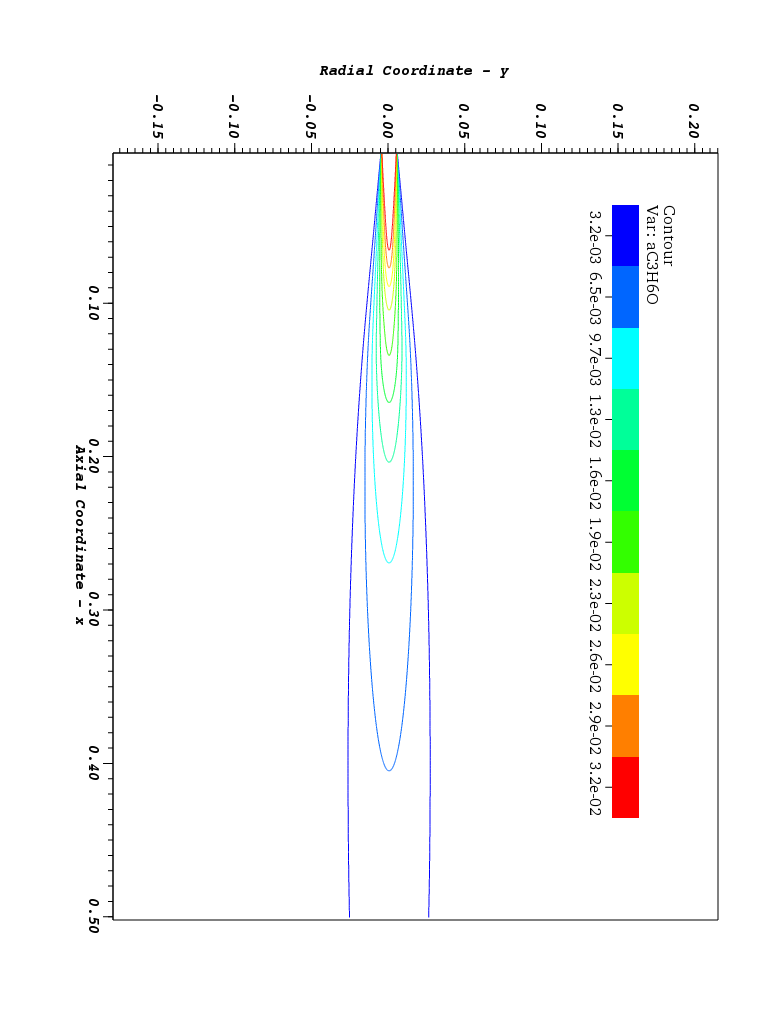
\includegraphics[height=0.9\textheight]{./figuras/appA2/visit_aC3H6O.png}
 \end{center}
 \caption{Mean of acetone vapor mass concentration - $\tilde{Y}_{ac}$. The computational domain is only half of the shown above, it is here mirrored for visualization purpose.}
 \label{fig: aa}
\end{figure}

\FloatBarrier
